% !TEX root = deckblatt4.tex
\section{Amplitudenmodulation}

\subsection{Aufgabenstellung}
Es sollte ein Nutzsignal auf ein Hochfrequenztes Tr\"agersignal aufmoduliert werden und anschlie\ss{}end im Frequneznbereich gemessen werden. Des weiteren mussten Berechneungen durchgef\"uhrt werden und mit den Messergebnissen verglichen werden.

\subsection{Zeitbereich}

\begin{figure}[H]
 \begin{center}
  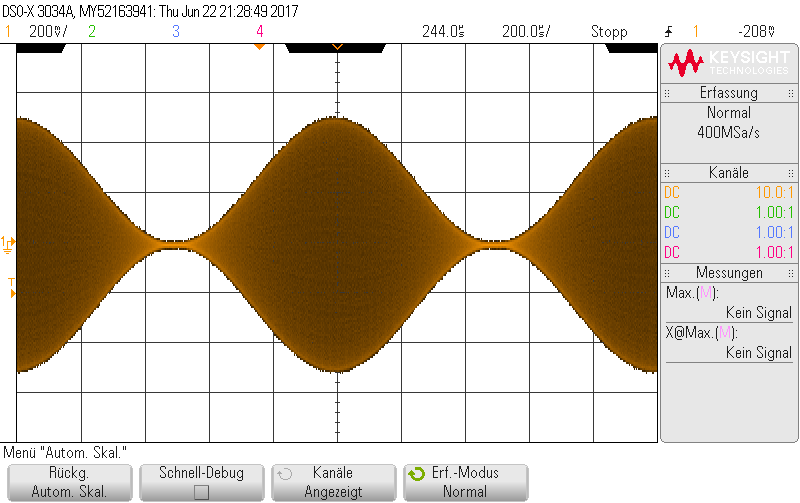
\includegraphics[height=6cm,width=12cm]{OsziBilder/bsp3_am_sin_time}
 \end{center}
 \caption{Zeitverlauf des AM-Singales, mit Sinus-Träger- und Nutzsignal}
\end{figure}

\begin{figure}[H]
 \begin{center}
  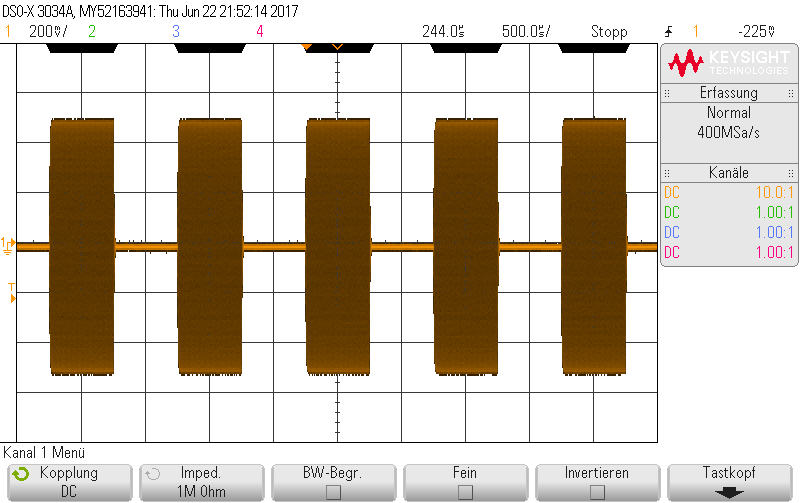
\includegraphics[height=6cm,width=12cm]{OsziBilder/bsp3_am_rect_time}
 \end{center}
 \caption{Zeitverlauf des AM-Signales, mit Sinus-Träger- und Rechteck-Nutzsignal}
\end{figure}

\subsection{Frequenzbereich}

\begin{figure}[H]
 \begin{center}
  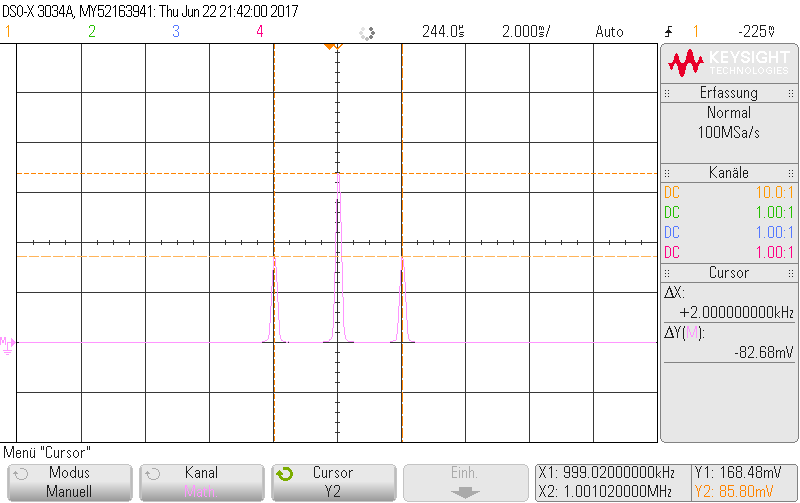
\includegraphics[height=6cm,width=12cm]{OsziBilder/bsp3_sin_rms_allCursor}
 \end{center}
 \caption{Spektraldarstellung des AM-Signales, mit Sinus-Träger- und Nutzsignal}
\end{figure}

\begin{figure}[H]
 \begin{center}
  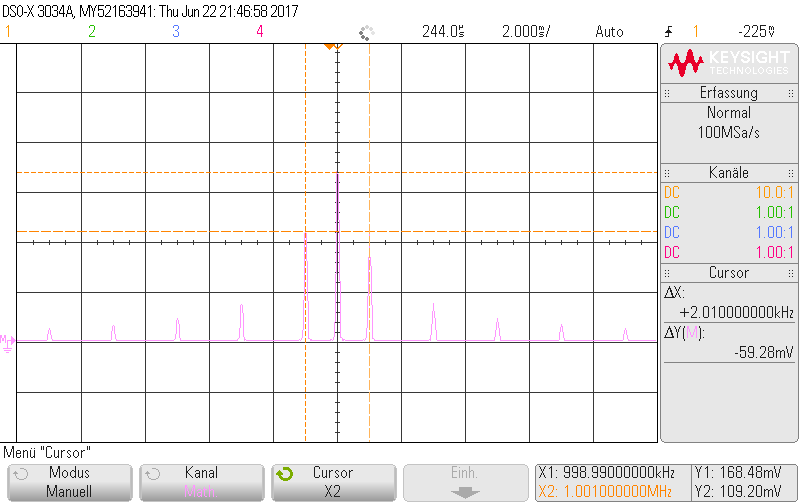
\includegraphics[height=6cm,width=12cm]{OsziBilder/bsp3_am_rect_rms_cursor}
 \end{center}
 \caption{Spektraldarstellung des AM-Signales, mit Sinus-Träger- und Rechteck-Nutzsignal}
\end{figure}

\subsection{Brechnungen}

\begin{figure}[H]
\textbf{Messwerte:} \centering \\
 \begin{minipage}[c]{.3\textwidth}
 \centering
  \begin{tabular}{c|c}
   $\hat{U}_{carrier}$ & $500mV$ \\ \hline
   $\hat{U}_{info}$ & $500mV$ \\ \hline
   $U_0$ & $0V$ \\ \hline
   $f_{carrier}$ & $1MHz$ \\ \hline
   $f_{info}$ & $1kHz$ \\ \hline
  \end{tabular}
  \caption{AM-Signal}
 \end{minipage}
 %
 \begin{minipage}[c]{.3\textwidth}
 \centering
  \begin{tabular}{c|c}
   $\hat{U}_{carrier}$ & $168,48mV$ \\ \hline
   $\hat{U}_{AM}$ & $85,80mV$ \\ \hline
   $f_{carrier}$ & $1MHz$ \\ \hline
   $f_{-1AM}$ & $999kHz$ \\ \hline
   $f_{1AM}$ & $1,001MHz$ \\ \hline
  \end{tabular}
  \caption{Sinus}
 \end{minipage}
 %
 \begin{minipage}[c]{.3\textwidth}
 \centering
  \begin{tabular}{c|c}
   $\hat{U}_{carrier}$ & $168,48mV$ \\ \hline
   $\hat{U}_{0AM}$ & $109,2mV$ \\ \hline
   $\hat{U}_{2AM}$ & $37,44mV$ \\ \hline
   $\hat{U}_{4AM}$ & $21,84mV$ \\ \hline
   $\hat{U}_{6AM}$ & $15,6mV$ \\ \hline
   $f_{carrier}$ & $1MHz$ \\ \hline
   $f_{0AM}$ & $1,001MHz$ \\ \hline
   $f_{2AM}$ & $1,003MHz$ \\ \hline
   $f_{4AM}$ & $1,005MHz$ \\ \hline
   $f_{6AM}$ & $1,007MHz$ \\ \hline
  \end{tabular}
  \caption{Rechteck}
 \end{minipage}
\end{figure}

\begin{center}
  \begin{align*}
    U_{carrier}(t) &= \hat{U}_{carrier} * cos(\omega_c t)\\
		   &= 0,5 * cos(10^6)\\ \\
    U_{info} &= \hat{U}_{info} * f_{info}(t)\\
	     &= 0,5  * cos(10^3)\\ \\
    U_{AM}(t) &= \frac{U_0 + U_{info}(t)}{U_0 + \hat{U}_{info}} * U_{carrier}\\
	      &= \frac{0 + 0,5  * cos(10^3)}{0 + 0,5} * 0,5 * cos(10^6)\\
	      &= 0,5 * cos(10^3) * cos(10^6)\\
	      &= 0,25 * (cos(0,999*10^6) + cos(1,001*10^6)\\
  \end{align*}
\end{center}
\noindent
Die berechneten Frequenzen stimmen exakt mit den Gemessenen überein. Bei den Amplitudenwerten gibt es jedoch abweichungen, allerdings
stimmt das Verhältnis von $0,5$ mit den Messwerten überein.\\
\\
Das Rechtecksignal besteht aus unendlich vielen Spektralkomponenten, w\"urde man nun mehrere Signale zur Daten\"ubertragung verwenden, so w\"urden eben diese Nebenkomponenten die Nachbar Kan\"ale st\"oren. Daher m\"sste das Signal vor der Abtastung mit einem Bandpass gefilter werden, um die Bandbreite des Signals zu begrenzen.\\
